\setlength{\footskip}{8mm}

\chapter{METHODOLOGY}

The methodology is structured into two parts. The first part involves a preliminary study (Study 1) conducted to determine the optimal parameters of the speller, while the second part (Study 2) focuses on examining the long-term viability of the trained ensemble TRCA model.

\section{Study 1: Preliminary Study}

\begin{figure}[h]
    \centering
    \caption{GUI design of hybrid speller.}
    \label{fig:speller-layout}
    \subfloat[\centering Distribution of 8 characters on the screen]{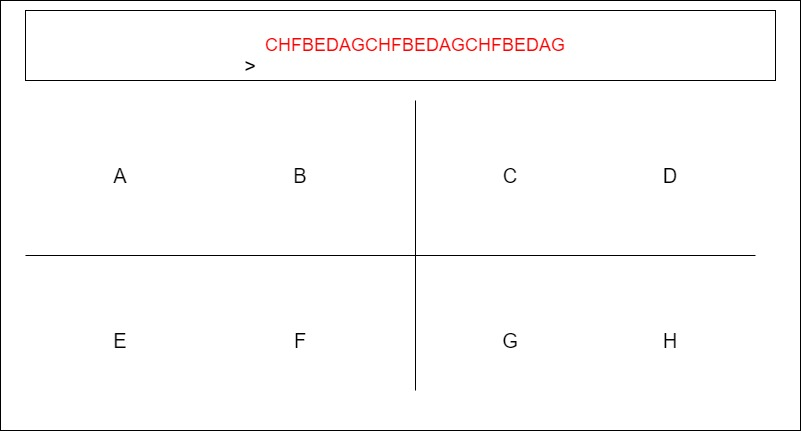
\includegraphics[width=0.45\textwidth]{figures/8-target-speller.jpg}}\hfill
    \subfloat[\centering Distribution of 12 characters on the screen]{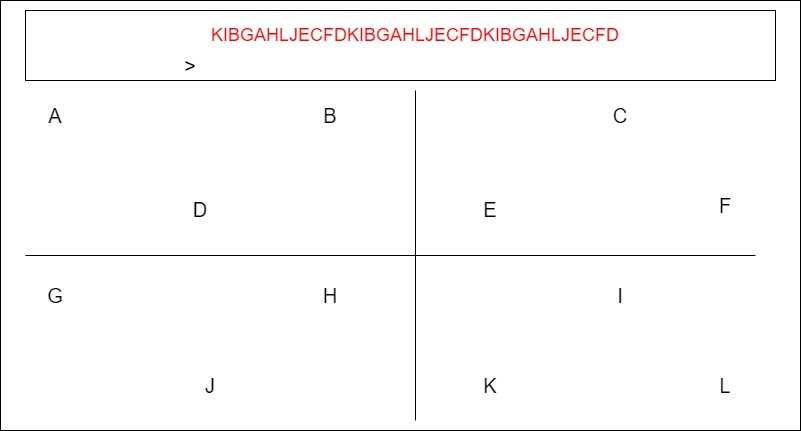
\includegraphics[width=0.45\textwidth]{figures/12-target-speller.jpg}}%
    \\
    \subfloat[\centering Distribution of 16 characters on the screen]{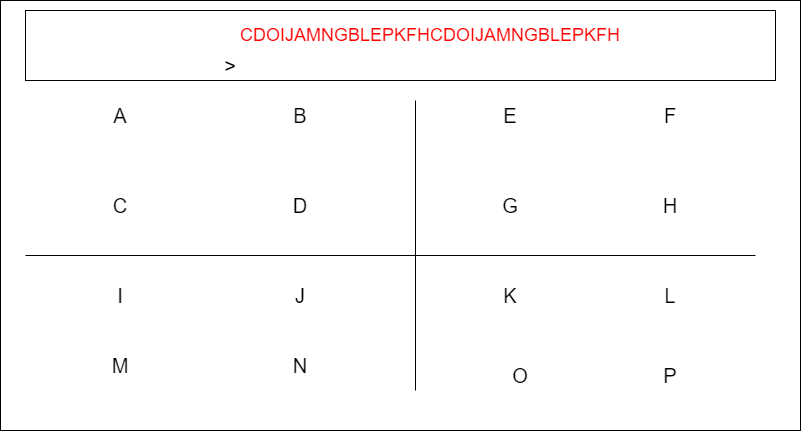
\includegraphics[width=0.45\textwidth]{figures/16-target-speller.png}}\hfill
    \subfloat[\centering The selected frequencies and initial phase for each sub-speller]{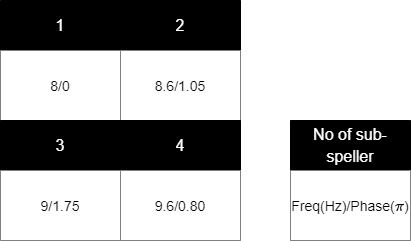
\includegraphics[width=0.45\textwidth]{figures/frequency-phase.png}}%
\end{figure}

This study focused on finding the optimal BCI speller parameters namely, (1) the number of targets ($C$), (2) flicker duration ($T_{\text{flicker}}$) and overlap ($O$) where \( 0 \leq O \leq 1 \) where \(0\) means no overlap and \(1\) means fully overlap, (3) flicker frequency ($F_c$) and phase ($P_c$) where $c \in C$, and (4) trial size per target ($S$). 
The range of targets is 8, 12, and 16, and organized into four sub-spellers with an equal amount of targets in each sub-speller as shown in Figure~\ref{fig:speller-layout}. 
The range of flicker duration is between 1 and 2 seconds paired with either no overlap or half overlap. Two sets of flicker frequencies and phases [8.0/0.00, 8.6/1.05, 9.0/1.75, 9.6/0.80] \textcolor{red}{cite which paper we copy} Hz and [12.4/0.00, 13.2/1.40, 14.0/0.80, 14.6/1.85] \textcolor{red}{cite which paper we copy} Hz were used in the experiment.
And, the effect of trial size ranges from 7 to 20 trials per target. 
The flicker size was constant at $100 \times 100$ pixels. 
The goal was to identify the most effective configuration to achieve reliable and accurate results.

\subsection{Participants}
A single participant (aged 26, female) with normal vision volunteered for this study.   

\subsection{Materials and Equipment}
EEG data were acquired using g.tec Unicorn Hybrid Black EEG Headset with a sampling rate of 250 Hz. 
The headset is equipped with eight electrodes (Fz, Cz, C3, C4, Pz, PO7, PO8, and Oz) based on the International 10/20 system. 
The Unicorn Suite Hybrid Black application was used to ensure that the electrodes were working correctly after the participant wore the cap. 
A conductive electro-gel was used to enhance the conductivity and stabilize the signal. 
The visual stimuli were presented on a 27-inch liquid-crystal display (LCD) monitor with a resolution of 1920 $\times$ 1080 with a refresh rate of 60 Hz.

The experiments were conducted in a controlled environment. 
To eliminate external influences, the room was darkened by covering the windows and creating an undisturbed ambiance. 
The experimental procedures were approved by the institutional review board at the Asian Institute of Technology.

The speller was developed using Python version 3.8.3. For recording and processing the signal, the MNE library version 1.3.0 was employed. 
Additionally, the BrainFlow library version 5.6.2 was utilized to analyze the EEG signals. 
The stimulation system was developed using PsychoPy version 3. 
In our study, we utilized the ensemble TRCA code, which was developed based on the methodology presented in the work by \cite{nakanishi2017enhancing}.
The code from the corresponding GitHub repository \url{https://github.com/mnakanishi/TRCA-SSVEP} was employed for our analysis.

\subsection{Data Collection}
\label{metho:data-collection}

One set of data is obtained from one session.
The data is collected in blocks design with breaks in between each block.
A block consists of $2 \times C$ number of trials. 
The number of blocks in one session \((B)\) is $\frac{S}{2}$. 
The duration of a break ($T_{\text{break}}$) varied depending on $C$ using the following logic.

\[ D_{\text{break}}=\begin{cases}
    30 \text{ if } C = 8 \\
    40 \text{ if } C = 12 \\
    60 \text{ if } C = 16 \\
\end{cases}\]

A trial consists of cue time ($T_\text{cue}$) and flickers. 
Time of a trial is \( T_\text{trial} = T_\text{cue} + T_\text{flicker} \times ( 1 + ((1 - O) \times (\frac{C}{4} - 1)) ) \). 
Thus, the duration of a single block can be calculated as \( T_{\text{block}} = 2C \times T_\text{trial} \).
Finally, a session time \( T_\text{session} \) can be calculated with \( (B \times T_\text{block}) + (B - 1) \times T_\text{break} \)

In a trial, \(T_\text{cue}\) is set to one second. 
During this second, a red box is displayed on the screen over the target indicating the specific target that the participant needed to focus on.
After that, a sequence of flickers following the order is presented.
Please note that the order is random once at the beginning of the project for each sub-speller of each target number \((C)\). 
These orders are used for all sessions.

\textcolor{red}{How is the target order?}
The order of the targets is random in every session.

\subsection{Task and procedure}

There are two types of sessions in our experiment: an offline session and an online session.
The data we obtain from an Offline session will be used to train the ensemble TRCA.
Subsequently, the trained model will be evaluated against the Online session.
The detail of how the model is obtained will be discussed later in Section~\ref{metho:models}

The preparation instruction was given to all participants.
It instructed the participants to omit the use of hair products (e.g. sprays or gels) in the morning of the experiment day, and avoid eating or drinking anything containing caffeine for at least 8 hours before the test.

For each offline session, the participant was asked to sit comfortably in a chair, facing a monitor positioned at a distance of approximately 60 cm measuring from screen to eyes.
The g.tec Unicorn Hybrid Black EEG Headset was put on together with monitoring the signal quality using the Unicorn Suite Hybrid Black application.
The instruction on how to perform the BCI speller was reminded again.
When ready, the data collection was started following Section~\ref{metho:data-collection}.
The data was obtained in a three-dimensional data \( ( C \times S, \texttt{n\_channels}, \texttt{n\_samples}) \) where  \texttt{n\_channels} is 8 and \texttt{n\_sample} is \(250 \times T_\text{trial} \)

\textcolor{red}{continue here}

In the online task, the experimental setup remained largely similar to the offline task. 
However, there was only a single block consisting of three trials for each target. 
Real-time predictions were generated using the previously trained and saved model. 
The system's output was displayed instantaneously on the screen, providing immediate feedback to the participant. 

\subsection{Preprocessing}
The raw EEG signals obtained during both the online and offline tasks underwent bandpass filtering within the frequency range of 1 to 92 Hz, with an additional notch filter at 50 Hz. For the ensemble TRCA decoding algorithm, a filterbank of [[(1, 92), (0, 100)], [(7, 92), (6, 100)]] was utilized. Apart from these steps, no additional preprocessing was applied to the EEG signals.

\subsection{Models}
\label{metho:models}
Ensemble Task-Related Component Analysis (TRCA) was used as the classification model.
\textcolor{red}{Using 5-cv. How to split, save best model.}

All these parameters of the speller were varied and different experiments were conducted. To assess the offline accuracy of the system, a stratified 5-fold cross-validation methodology was employed. The model yielding the best performance across the folds was saved and utilized in the online experiment.

\subsection{Evaluation metrics}
Offline accuracy, online accuracy and information transfer rate (ITR) were used as the evaluation metrics. The offline accuracy of the system was computed using a stratified 5-fold cross-validation. Online accuracy was calculated by using the number of correct and incorrect prediction done by the speller.

\[
\text{{ITR}} = \left[\log_2 N + P \log_2 P + (1 - P) \log_2 \left(\frac{{1-P}}{{N-1}}\right)\right] \times \left(\frac{{60}}{{T}}\right)
\]

\subsection{Result and Discussion}

\subsubsection{Effect of Number of Samples}

Based on the initial experimental results with a single subject, it was observed that a higher number of data samples per class led to improved outcomes. 
Table \ref{tab:comparaision_no_of_samples} shows the positive effect of increasing the number of samples on the overall results. Specifically, when comparing the 8 target speller, the offline accuracy noticeably improved when the number of samples was increased from 12 to 15. Moreover, for the 16 target speller, similar improvements were observed as the offline accuracy increased when the number of samples was raised from 7 to 15. However, individuals can experience fatigue during prolonged data collection sessions, so we decided to set the number of samples per class to 20. To achieve this, we divided the experiment into 10 blocks, with 2 trials for each character within each block.

\begin{table}[h]
\small
\caption{Comparison of Number of Trials}
\label{tab:comparaision_no_of_samples}
\begin{tabular}{@{}p{1.2cm} p{2.5cm} p{1.5cm} p{2cm} p{1.7cm} p{1.5cm} p{2cm} p{2cm}@{}}
\toprule
No of Stimuli  & Flicker   duration (sec) & Trials & Overlap & Acc\textsubscript{off}(\%)  \\ \midrule
8                    & 3                        & 12                             & 0                       & 75                      \\
8                   & 3                        & 15                          & 0                       & 79                       \\
16                 & 2                        & 7                          & 0.5                     & 57.23                        \\
16                 & 2                        & 15                        & 0.5                     & 72.50                       \\\bottomrule
\end{tabular}
\end{table}

\subsubsection{Effect of Stimuli Time and Overlap}

Table \ref{tab:comparison_stimuli_time_overlap} shows the comparison of accuracy when stimuli time and overlap were varied. For the 8 target speller, the highest online and offline accuracy was achieved with a flicker duration of 2 seconds and a 0.5 overlap of stimuli. As we decreased the flicker duration to 1 second with no overlap and 1 second with 0.5 overlap, the accuracy decreased.

However, for the 16 target speller, even with the 2-second stimuli and no overlap, the accuracy obtained was not significantly high. Furthermore, reducing the stimuli flicker duration to 1 second with no overlap and 1 second with 0.5 overlap further degraded the performance.

Finally, when considering the 12 target speller, a flicker duration of 2 seconds with a 0.5 overlap and 20 trials of each character resulted in an acceptable outcome.

\begin{table}[h]
\small
\caption{Comparison of Stimuli Time and Overlap}
\label{tab:comparison_stimuli_time_overlap}
\begin{tabular}{@{}p{1.2cm} p{2.5cm} p{2cm} p{1.8cm} p{1.7cm} p{1.5cm} p{2cm} p{2cm}@{}}
\toprule
No of Stimuli  & Flicker   duration (sec) & Trials & Overlap & Acc\textsubscript{off}(\%) \\ \midrule
8                      & 2                        & 20                            & 0.5                     & 90                     \\
8                    & 1                        & 20                             & 0                       & 88                 \\
8                  & 1                        & 20                          & 0.5                     & 81                     \\
16                  & 2                        & 15                          & 0.5                     & 72.50                     \\
16                & 1                        & 15                            & 0                       & 44.58 \\
16 &1  & 15                           & 0.5                     & 57                       \\
12             & 2                      & 20                         & 0.5           & 79               \\\bottomrule
\end{tabular}
\end{table}

\subsubsection{Effect of Frequency range}

Table \ref{tab:comparison_freq_range} show the experiment conducted in two different days. All other parameters are kept constant except the frequency and phase of the subspeller. It was found that the performance of the speller was better when we used the lower frequency range.

\begin{table}[ht]
\small
\caption{Comparison of Frequency range}
\label{tab:comparison_freq_range}
\begin{tabular}{@{}p{1.2cm} p{1.5cm} p{1.0cm} p{1.8cm} p{1.8cm} p{3.5cm} p{1.5cm} p{1.5cm}@{}}
\toprule
No of Stimuli & Flicker   duration (sec) & Blocks & Trial/Block & Overlap(\%) & Freq (Hz)              & Acc\textsubscript{off}(\%)     \\ \midrule
16            & 2                        & 15           & 16                      & 0.5                     & {[}8,8.6,9,9.6{]}             & 72.5                        \\
16            & 2                        & 15           & 16                      & 0.5                     & {[}8,8.6,9,9.6{]}             & 73.33                      \\
16            & 2                        & 15           & 16                      & 0.5                     & {[}12.4,13.2,14.0,14.6{]}     & 58.33                     \\
16            & 2                        & 15           & 16                      & 0.5                     & {[}12.4,13.2,14.0,14.6{]}     & 61.25                      \\ \bottomrule
\end{tabular}
\end{table}


\begin{table}[ht]
\small
\caption{Comparison of Frequency range}
\label{tab:comparison_freq_range}
\begin{tabular}{@{}p{1.2cm} p{2.5cm} p{1.8cm} p{1.8cm} p{4cm} p{2.5cm}@{}}
\toprule
No of Stimuli & Flicker duration (sec) & Trials & Overlap(\%) & Freq (Hz)              & Acc\textsubscript{off}(\%)     \\ \midrule
16             & 2                      & 15        & 0.5         & {[}8,8.6,9,9.6{]}             & 72.92$\pm$0.53 \\
16            & 2                      & 15        & 0.5       &{[}12.4,13.2,14.0,14.6{]}             & 59.79$\pm$1.75\\
\bottomrule
\end{tabular}
\end{table}

Moreover,it is known that not all participants can perform equally well when it comes to BCI experiment. Therefore, to accommodate a broader range of users, we selected the parameters as follows: flicker duration of 2 seconds, 0.5 overlap, 10 blocks, and 2 trials per character per block. This selection aimed to ensure that the system remains usable for a greater number of participants.

\subsubsection{Other observations}
Along the experiments, we also informally altered some parameters and here are some note worthy points to know:

\textbf{Darker environment:} We discovered that conducting the offline experiment in a darker environment yielded better training data. This allowed us to train the ensemble TRCA model with higher quality data, resulting in improved performance. However, once the model was trained with quality data, we observed that online experiments were less affected by variations in lighting conditions. 

\textbf{Time alignment:} In our studies, we made an additional observation regarding the alignment of EEG signals in online experiments. We noticed that the received EEG signals during online sessions may not be perfectly time-aligned with the training data. To address this issue, we experimented with adding a specific offset to the online EEG signals.

By introducing this offset, we aimed to align the online signals more closely with the timing patterns learned during training, thereby improving the overall performance of the system. Remarkably, we found that incorporating the offset proved to be beneficial, resulting in enhanced results during online experiments.

This finding highlights the importance of accounting for temporal discrepancies between training and online data in BCI systems. By introducing the appropriate offset, we were able to mitigate the potential misalignment and optimize the system's performance. This further underscores the need for careful calibration and synchronization measures when deploying BCI technologies in real-time applications.

\section{Study 2: Long-term viability Study}

This study was undertaken to assess the long-term viability of the trained ensemble TRCA model. The objective was to investigate whether the model remains effective and practical after a considerable time.

\subsection{Participants}

A total of twenty-three healthy individuals with normal or corrected-to-normal vision participated in the final experiments, which were divided into three sessions.

In the first session, participants completed an offline experiment using the 8 target speller, followed by an online experiment. Out of the initial twenty-three participants, fourteen individuals demonstrated proficient performance on the 8 target speller, achieving a classification accuracy of 70\% or higher on the best fold of the offline experiment. To evaluate the classification accuracy, stratified 5-fold cross-validation was applied, and the model from the best fold was selected and saved for further analysis. Participants who did not meet the performance criterion during the first session were excluded from subsequent sessions.

 Prior to participating in the experiments, participants were provided with comprehensive information regarding the study. They were fully informed about the experiment's objectives, procedures, potential risks, and their rights as participants. All participants voluntarily consented to participate by signing the informed consent form, affirming their understanding and agreement to take part in the study.


\subsection{Speller}

Three different spellers were used for the experiments to compare their performance, feasibility and effectiveness.

The first speller consists of 8 targets. The design of the 8 target speller is shown in Figure \ref{fig:speller-layout}.The design consists of 4 sub speller with 2 character each in the sub speller. The layout consists of 2 $\times$ 4 matrix showing 8 characters in a white background. The characters of the speller were highlighted by a visual flicker of size 100 $\times$ 100 pixels in a fixed random sequence. The stimulus duration for each character was set to 2 s. The flickering patterns of the stimuli had a 0.5 overlap, adding a degree of continuity to the visual presentation. To facilitate target selection, the targeted characters were distinctly highlighted by a red cue box. This cue box, also of size 100 $\times$ 100 pixels, remained visible for 1 second before the stimuli began flickering.

The sampled sinusoidal stimulation method \cite{chen2014high} was used to present the visual flickers. JFPM method \cite{chen2015high} was used to determine the frequencies and phases of the six flickering stimuli. Similar to \cite{xu2020implementing} 4 flickering frequencies were selected for the visual stimuli: 8 Hz, 8.6 Hz, 9 Hz, 9.6 Hz with phases 0, 1.05, 1.75, 0.80 respectively. 

The second speller consists of 12 targets. The design of the 12 target speller is shown in Figure \ref{fig:speller-layout}. It also consists of 4 sub speller and each sub speller had 3 characters each. All other parameters were consistent with the 8 target speller.Also the characters within the sub-speller utilize the same frequency and phase as those in the 8-target speller.

The third speller consists of 16 targets. The design of the 16 target speller is also shown in the Figure \ref{fig:speller-layout}. It consists of 4 $\times$ 4 matrix of English alphabetical characters presented within 4 sub spellers. All other parameters remain consistent with the other spellers.



\subsection{Task and procedure}
The participants were instructed to sit in front of a monitor screen, at a distance of approximately 60 cm. The monitor displayed a layout consisting of English alphabets, organized in a specific manner as depicted in Figure \ref{fig:speller-layout}. 

The participants were given a straightforward task: to maintain their focus on the targeted character highlighted by the cue with minimal blinking and mentally retain the target character throughout the flickering process. This approach aimed to ensure sustained focus and cognitive engagement during the task.


\begin{figure}
  \centering
  \caption{A participant performing online experiment}
  \label{fig:online-participant}
  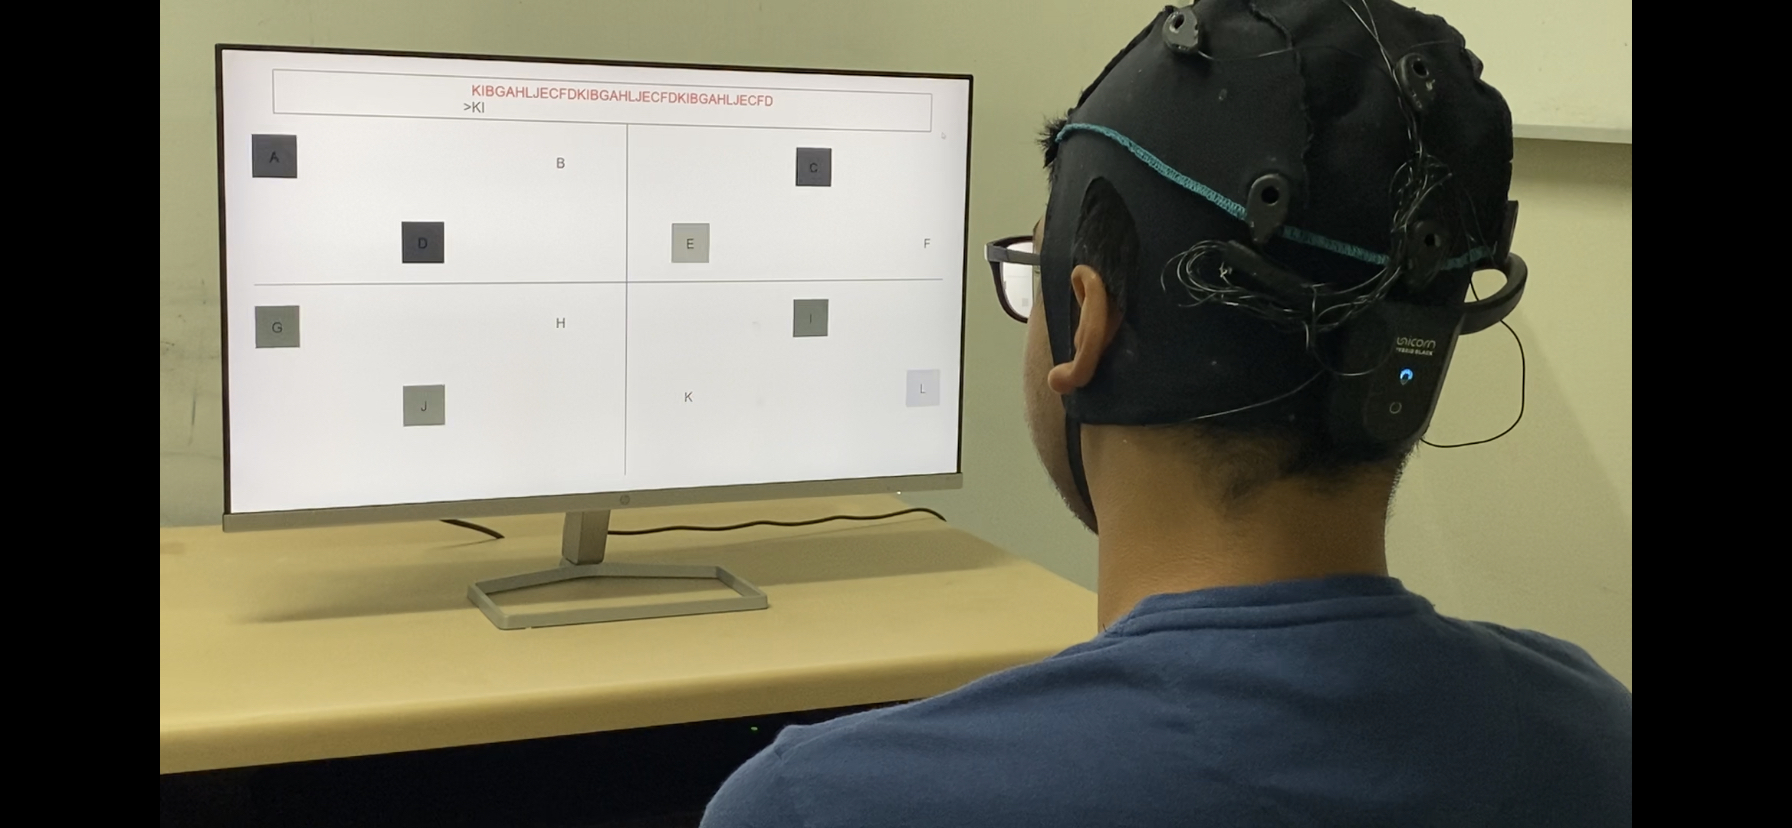
\includegraphics[width=0.8\textwidth]{figures/experimental-setup.PNG}
\end{figure}

The experiment consisted of three sessions, each involving different combinations of offline and online experiments.

During the first session, the 8-target speller was used, and participants took part in an offline experiment, followed by an online experiment. Similarly, the second session involved the utilization of the 12-target speller, following the same offline and online experiment structure as the first session.

The third session solely comprised online experiments, with one session dedicated to the 8-target speller and another session dedicated to the 12-target speller. Notably, the same model saved during the first and second sessions was utilized in the third session. After a minimum gap of one day following the second session, participants proceeded to the third session. This session aimed to assess the durability and stability of the trained model, examining its performance even after a gap of several days. By conducting experiments on different days, the study sought to evaluate the robustness and generalizability of the model over time and under varying conditions.

Further elaboration on the online and offline experiments is provided below.

\subsubsection{Offline Experiment}
The offline experiment was divided into 10 blocks. The character to be selected was indicated by a red outline for 1 second. 

In the 8-target speller, each block of the offline experiment consisted of 16 trials, with 2 trials allocated to each of the 8 stimuli. The duration of each trial was 3 seconds. A 30-second break was provided between each block. Consequently, the entire offline experiment lasted approximately 12.5 minutes for each subject.

Similarly, in the 12-target speller, each block comprised 24 trials, with 2 trials assigned to each of the 12 stimuli. Each trial lasted for 4 seconds. A 40-second break was given between each block. Hence, the total duration of the offline experiment was approximately 22 minutes for each subject.

The 16-target speller offers a wider range of stimuli for participants to interact with. Each block in the 16-target speller comprises 32 trials, with 2 trials assigned to each of the 16 stimuli. Each trial was took 5 sec to complete. Following each block, there is a 60-second break to allow participants to rest and prepare for the next block. With a total of 10 blocks in the offline experiment, the entire duration of the 16-target speller is approximately 36.67 minutes for each subject. 

\begin{equation}
    T_{\text{total}} = N_{\text{blocks}} \times (N_{\text{trials}} \times N_{\text{chars}}) \times T_{\text{trial}} + (N_{\text{blocks}} - 1) \times T_{\text{break}}
\end{equation}
T\textsubscript{\text{total}} is the total time.\\
N\textsubscript{\text{blocks}} is the number of blocks.\\
N\textsubscript{\text{trials}} is the number of trials per character.\\
N\textsubscript{\text{chars}} is the number of characters.\\
T\textsubscript{\text{trial}} is the time taken per trial.\\
T\textsubscript{\text{break}} is the block break time.\\
    

\subsubsection{Online Experiment}
The online cue-guided spelling experiment consisted of a single block with 3 trials of each character. For 8 target speller, each trial lasted for 3 sec. For 12 target speller, each trial lasted for 4 sec with 0.5 percentage overlap of stimuli flicker. The cue duration for online experiment was about 2 sec. The results of each trial were promptly displayed on the screen in real time, providing instant feedback. 

\subsection{Evaluation metrics}
Same metrics have been used as in the study 1.

\subsection{Result and Discussion}  

Table \ref{tab:eight-target-comparison} and Table \ref{tab:twelve-target-comparison} shows the offline accuracy, online accuracy and online accuracy after at least 1 day for the 8 target speller and 12 target speller respectively. While the average accuracy decreased in the third session for the 8 target speller, it is important to note that individual participants displayed varied performance. Some participants demonstrated improvement in accuracy during the third session, while others experienced a decline. However, in the case of the 12-target speller, the overall accuracy increased yet it still remained true that certain participants exhibited enhanced performance, while others saw a decrease. 

The absence of a consistent or clear pattern suggests that performance is not directly influenced by the passage of time. Instead, it is plausible that factors such as the participant's level of focus on a given day, their state of mind, and the amount of concentration exerted could have contributed to the observed variations in results. This result points out that combining recordings from multiple sessions could be a viable approach. It allows for a larger sample size without subjecting the user to excessive fatigue. By including data from different sessions, the model benefits from a more extensive and diverse dataset, capturing a wider range of conditions and performance variations.

In order to investigate the potential for improvement in participants' performance with the BCI speller, we conducted a specific training session with one participant. The objective was to determine if targeted training could enhance their ability to utilize the speller effectively.

During the training, various techniques were employed to assist the participant in maintaining focus. They were instructed to employ strategies such as counting the number of stimuli flickers and continuously mentally rehearsing the alphabet to sustain concentration. Furthermore, the participant exclusively participated in an online SSVEP experiment, employing FBCCA (frequency-based canonical correlation analysis) for classification. The online system provided real-time feedback, allowing the participant to ascertain whether their focus-enhancing techniques were effective.

The training spanned three consecutive days, with the participant actively engaging in the experiment. Following the completion of the training period, three offline experiments were conducted to evaluate the participant's performance. Surprisingly, despite the intensive training, no significant improvement in performance was observed.

These findings suggest that, in this particular case, the employed training techniques and the duration of the training period did not lead to notable enhancements in the participant's ability to utilize the BCI speller effectively. It highlights the complexity of individual variability in BCI performance and underscores the need for further investigation and experimentation to develop effective training strategies for improving BCI user performance. 


\begin{table}[h]
\small
\caption{Comparison of accuracy of 8 target speller offline and online}
\label{tab:eight-target-comparison}
\begin{tabular}{@{}p{1.8cm}p{2cm}p{2cm}p{2.2cm}p{2cm}p{2.2cm}p{2cm}@{}}
\toprule
Subject & Offline(\%) & Best Fold(\%) & Online 1(\%) & ITR(bits/min) & Online 2(\%) & ITR(bits/min) \\ \midrule
S1      & 83.75       & 87.50        & 88.00        & 32             & 91.60        & 35.22 \\
S2      & 85.00       & \textbf{95.83}        & 81.00        & 26.47          & 87.00        & 31.16 \\
S3      & 70.00       & 79.16        & 68.75        & 18.39          & 62.50        & 14.89 \\
S4      & 76.66       & 83.33        & 56.25        & 11.74          & 66.66        & 17.18 \\
S5      & 74.16       & 83.33        & 68.75        & 18.39          & \textbf{100.00}       & \textbf{44.97} \\
S6      & 85.62       & 87.50        & 93.75        & 37.3           & 87.50        & 31.58 \\
S7      & 83.12       & 93.75        & 93.75        & 37.3           & 95.83        & 39.49 \\
S8      & 87.50       & 90.62        & 87.50        & 31.58          & 95.83        & 39.49 \\
S9      & 70.60       & 81.25        & \textbf{100.00}       & \textbf{44.97}          & 70.80        & 19.63 \\
S10     & 73.00       & 81.25        & 91.00        & 34.66          & 70.00        & 19.15 \\
S11     & 60.00       & 71.87        & 83.33        & 28.22          & 75.00        & 22.30 \\
S12     & 68.12       & 81.25        & 87.50        & 31.58          & 83.33        & 28.23 \\
S13     & 80.00       & 90.62        & 87.50        & 31.58          & 54.00        & 10.70 \\
S14     & \textbf{90.00}       & \textbf{95.83}        & 91.00        & 34.66          & 87.50        & 31.58 \\
\midrule
S15     & 63.75       & 68.75        & -             & -              & -             & - \\
S16     & 48.00       & 56.25        & -             & -              & -             & - \\
S17     & 45.00       & 56.25        & -             & -              & -             & - \\
S18     & 47.00       & 59.37        & -             & -              & -             & - \\
S19     & 11.25       & 18.75        & -             & -              & -             & - \\
S20     & 34.50       & 43.75        & -             & -              & -             & - \\
S21     & 16.00       & 25.00        & -             & -              & -             & - \\
S22     & 27.00       & 34.37        & -             & -              & -             & - \\
S23     & 45.00       & 56.25        & -             & -              & -             & - \\
\bottomrule

\multicolumn{7}{l}{\footnotesize\textit{Note:} 'Online 2' refers to the online accuracy obtained online at least one day later}
\end{tabular}
\end{table}

\begin{table}[h]
\small
\caption{Comparison of accuracy of 8 target spellers offline and online}
\label{tab:eight-target-comparison}
\begin{tabular}{@{}p{1.8cm}p{2cm}p{2cm}p{2.2cm}p{2cm}p{2.2cm}p{2cm}@{}}
\toprule
Subject & Offline(\%) & Best Fold(\%) & Online 1(\%) & ITR(bits/min) & Online 2(\%) & ITR(bits/min) \\ \midrule
S1      & 83.75       & 87.50        & 88.00        & 32             & 91.60        & 35.22 \\
S2      & 85.00       & 95.83        & 81.00        & 26.47          & 87.00        & 31.16 \\
S3      & 70.00       & 79.16        & 68.75        & 18.39          & 62.50        & 14.89 \\
S4      & 76.66       & 83.33        & 56.25        & 11.74          & 66.66        & 17.18 \\
S5      & 74.16       & 83.33        & 68.75        & 18.39          & \textbf{100.00}       & \textbf{44.97} \\
S6      & 85.62       & 87.50        & 93.75        & 37.3           & 87.50        & 31.58 \\
S7      & 83.12       & 93.75        & 93.75        & 37.3           & 95.83        & 39.49 \\
S8      & 87.50       & 90.62        & 87.50        & 31.58          & 95.83        & 39.49 \\
S9      & 70.60       & 81.25        & \textbf{100.00}       & \textbf{44.97}          & 70.80        & 19.63 \\
S10     & 73.00       & 81.25        & 91.00        & 34.66          & 70.00        & 19.15 \\
S11     & 60.00       & 71.87        & 83.33        & 28.22          & 75.00        & 22.30 \\
S12     & 68.12       & 81.25        & 87.50        & 31.58          & 83.33        & 28.23 \\
S13     & 80.00       & 90.62        & 87.50        & 31.58          & 54.00        & 10.70 \\
S14     & \textbf{90.00}       & \textbf{95.83}        & 91.00        & 34.66          & 87.50        & 31.58 \\ \midrule
Mean$\pm$Std & 77.68 $\pm$ 8.70 & 85.94 $\pm$ 6.96 & 84.15 $\pm$ 11.90 & 29.92 $\pm$ 9.74 & 80.00 $\pm$ 14.50 & 28.02 $\pm$ 9.78 \\ \bottomrule

\multicolumn{7}{l}{\footnotesize\textit{Note:} 'Online 2' refers to the online accuracy obtained online at least one day later}
\end{tabular}
\end{table}





\begin{table}[h]
\small
\caption{Comparison of accuracy of 12 target speller offline and online}
\label{tab:twelve-target-comparison}
\begin{tabular}{@{}p{1.8cm}p{2cm}p{2cm}p{2.2cm}p{2cm}p{2.2cm}p{2cm}@{}}
\toprule
Subject & Offline (\%) & Best Fold (\%) & Online 1 (\%) & ITR(bits/min) & Online 2 (\%) & ITR(bits/min) \\ \midrule
S1      & 72.00        & 77.77          & 70.00         & 19.99            & 83.33         & 28.30 \\
S2      & 41.67        & 47.22          & -             & -                & -             & - \\
S3      & 57.50        & 58.33          & 44.44         & 8.06             & 58.33         & 13.96 \\
S4      & 46.77        & 54.16          & 44.44         & 8.06             & 50.00         & 10.26 \\
S5      & 62.91        & 72.91          & 55.50         & 12.65            & 66.66         & 18.16 \\
S6      & \textbf{84.50}        & \textbf{90.62}          & 94.33         & 36.90            & 83.33         & 28.30 \\
S7      & 81.66        & 87.50          & 72.20         & 21.25            & 72.22         & 21.26 \\
S8      & 82.50        & 87.50          & \textbf{94.44}         & \textbf{36.99}            & \textbf{97.20}         & \textbf{39.65} \\
S9      & 75.00        & 87.50          & 86.77         & 30.76            & 77.77         & 24.62 \\
S10     & 58.33        & 64.58          & 63.88         & 16.70            & 61.11         & 15.31 \\
S11     & 53.00        & 60.41          & 72.22         & 21.26            & 47.77         & 9.35 \\
S12     & 75.55        & 80.55          & 86.50         & 30.56            & 75.00         & 22.91 \\
S13     & 53.75        & 56.25          & 52.77         & 11.44            & 58.33         & 13.96 \\
S14     & 78.75        & 87.50          & 69.44         & 19.68            & 86.00         & 30.20 \\ \bottomrule
Mean$\pm$ Std & 65.99$\pm$14.28 & 72.34$\pm$15.11 & 69.76$\pm$17.33 & 25.24$\pm$10.42 & 70.54$\pm$14.98 & 24.51$\pm$10.04 \\ \bottomrule
\multicolumn{7}{l}{\footnotesize\textit{Note:} 'Online 2' refers to the online accuracy obtained at least one day later}
\end{tabular}
\end{table}

\begin{table}[h]
\small
\caption{Comparison of accuracy of 16 target spellers offline and online}
\label{tab:sixteen-target-comparison}
\begin{tabular}{@{}p{1.8cm}p{2cm}p{2cm}p{2.2cm}p{2cm}p{2.2cm}p{2cm}@{}}
\toprule
Subject & Offline (\%) & Best Fold (\%) & Online 1 (\%) & ITR(bits/min) & Online 2 (\%) & ITR(bits/min) \\ \midrule
S1      & 39.37        & 45.31          & 18.75         & 1.29             & -             & - \\
S6      & \textbf{67.50}        & \textbf{73.43}          & 34.37         & 5.08             & -             & - \\
S12     & 60.31        & 68.75          & \textbf{71.87}         & 20.43            & 59.37         & 14.38 \\ \bottomrule
Mean$\pm$ Std & 55.06$\pm$13.49 & 62.16$\pm$13.51 & 41.66$\pm$27.08 & 8.26$\pm$9.34 & 59.37$\pm$0.00 & 14.38$\pm$0.00 \\ \bottomrule
\multicolumn{7}{l}{\footnotesize\textit{Note:} 'Online 2' refers to the online accuracy obtained at least one day later}
\end{tabular}
\end{table}



\cite{9618750}
\cite{8104195}
\cite{brennan2015accessing}